\section{CERN and the Large Hadron Collider}
The \textit{organisation européenne pour la recherche nucléaire} or CERN conducts the world's frontier particle physics experiments. 
Scientists at CERN represent numerous countries who work together for a greater understand of the universe. 
CERN hosts the Large Hadron Collider (LHC), currently the largest particle collider in the world. The LHC 27 km in circumference and holds eight experimental caverns 150 meters underneath the earth. Accelerator physicists and engineers strive to provide high energy collisions along these eight sites. More than 1500 superconducting magnets to steer and focus the accelerating protons. 
The beams are brought into collision at the four caverns where the experiments are sited.
%Crossing points facilitated by crab cavities force these particles to cross, collide, and interact at the caverns where the experiments take data. 
%Multiple campaigns for particle physics are done such as low intensity fills, lead-lead collisions, and proton collision. 
The LHC is capable of colliding both protons and heavy ions. 
The Compact Muon Solenoid (CMS) is the general purpose detector located at collision point 5(P5) in Cessy, France ~\cite{Bruning:782076}. 

\begin{figure}[ht!b]
  \centering
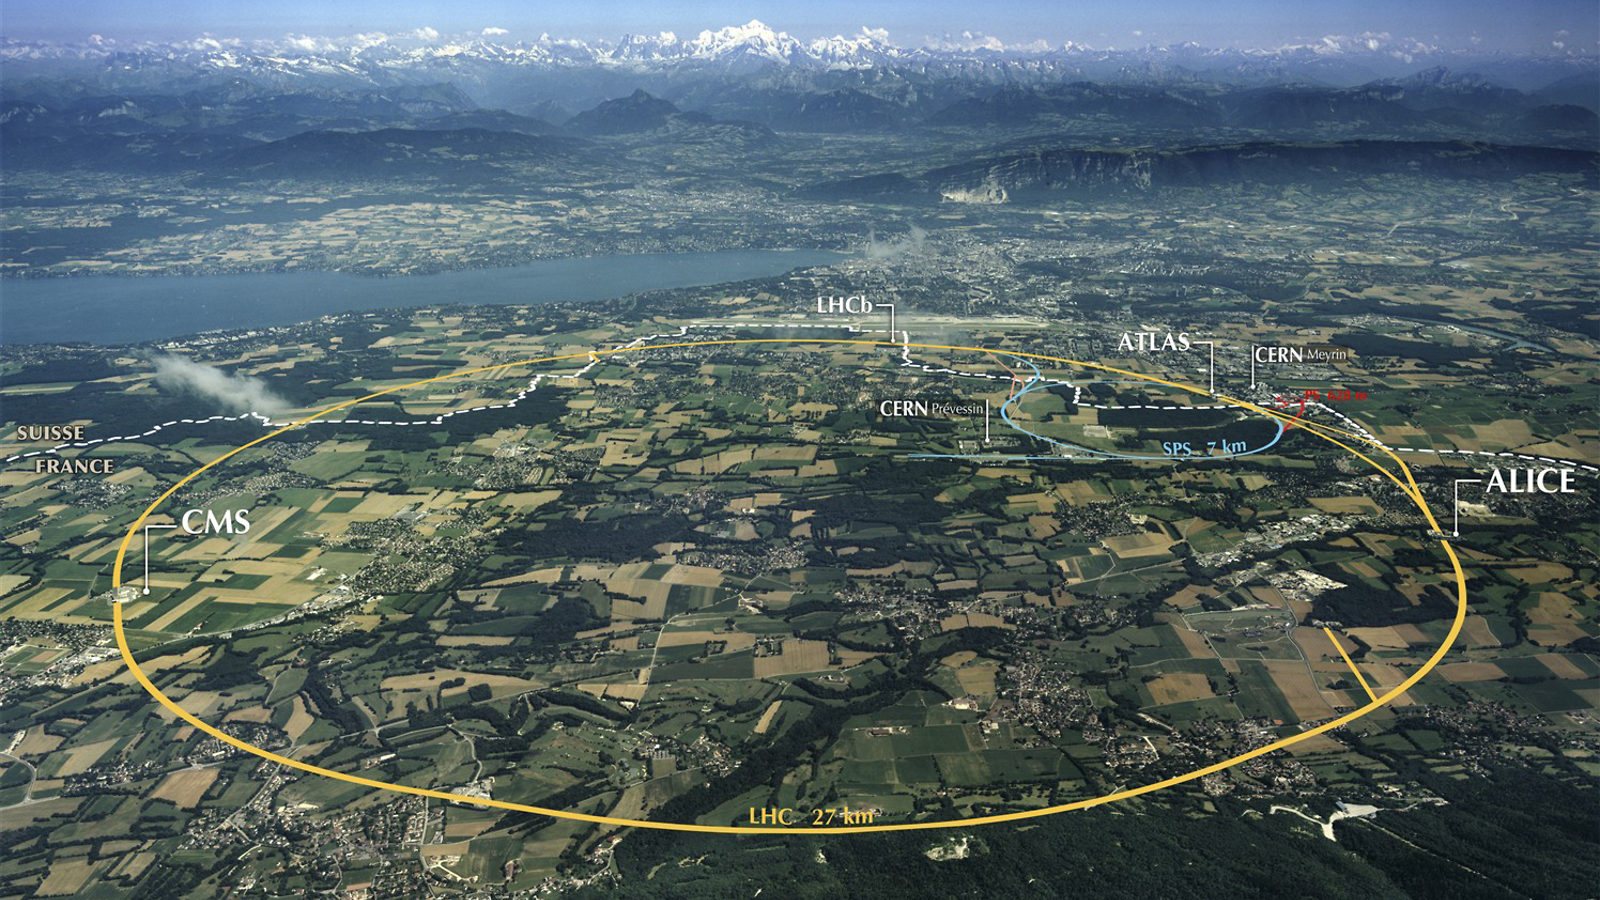
\includegraphics[width=0.75\textwidth]{figures/LHC_map-s.jpg}    
    \caption{\label{fig:lhc} Overview of the Large Hadron Collider spanning Switzerland and France - Maximilien Brice, CERN }
\end{figure}

\section{The Compact Muon Solenoid detector}
At around 14,000 tonnes, the CMS detector may not seem like it would be compact; however, it is quite dense. 
%fix 
As shown in the diagram, the detector contains many sub-detectors housed within a powerful solenoid magnet. At a diameter of 6 meters, a combined weight of 12,500 tonnes, and a field of 3.8 Tesla, the solenoid is the central feature of the Compact Muon Solenoid (CMS) \ref{fig:cmsdet}.
\begin{figure}[!htb]
\begin{center}
\includegraphics[width=0.75\textwidth]{Figures/cmsDet.png}
\caption{\label{fig:cmsdet}The CMS detector full 3D image with all subsystems labeled}
\end{center}
\end{figure}
 Within the solenoid volume, there is the
silicon pixel and strip tracker, a lead tungstate crystal 
electromagnetic calorimeter (ECAL), and a brass plus scintillator 
hadron calorimeter (HCAL). Each tracker and calorimeter comprises a barrel and two endcap 
sections. Forward calorimeters extend the pseudorapidity ($\eta$)
coverage provided by the barrel and endcap detectors. 
Muons are detected in gas-ionization chambers embedded 
in the steel flux-return yoke outside the solenoid.

A coordinate system centered on the nominal collision point is adopted. 
The $y$-axis points vertically outward toward the sky, the $x$-axis tangent to the Earth, and the $z$-axis along the direction of the beam pipe. The azimuthal angle $\phi$ and the radial coordinate $r$ in the $x$ and $y$ plane, and the polar angle $\theta$ measured from the $z$ axis are typically used to denote space points. 
Often pseudorapidity, defined by
\begin{equation}\eta = - \ln \tan(\theta/2)\end{equation}  
 is used to describe the angular distance from the beam pipe. 

%From the central interaction point, the CMS detector hosts
%the silicon pixel and strip tracker, the lead tungstate crystal electromagnetic
%calorimeter (ECAL), and the brass-scintillator hadron calorimeter (HCAL),
%each composed of a barrel and two endcap sections. The silicon pixel and tracking systems as well as
%the calorimeters are contained within the solenoid volume.  %cite

%The nominal $\Pp\Pp$ bunch crossing rate at the LHC is 40\unit{MHz}. This rate would be too extreme for any data taking system. In order to reduce the rate of events that are recorded for offline analysis, events of interest are selected using a two-step trigger system~\cite{Khachatryan:2016bia}.
%The first level (L1) is composed of custom built electronics which makes use of
%high speed optical links and large Field Programmable Gate Arrays (FPGAs). 

%L1 reduces the event rate from the nominal bunch crossing to a rate of aroun 100\unit{kHz} within a time interval of less than 3.5\mus.
%L1 reduces the rate from 40 MHz to 100 kHz.

%The second level, known as the High Level Trigger (HLT), consists of a farm of 
%generic processors running a version of the full event reconstruction software that
% has been optimized for fast processing. The HLT reduces the event rate to about
%1\unit{kHz} before data storage.

%Since the 2012 data taking, significant upgrades of the L1 trigger 
%have benefited this analysis, especially in the final state with two semi-hadronically decaying 
%$\Pgt$ leptons, denoted as $\tauh$.  
%These upgrades improved the $\tauh$ identification at L1 by giving more flexibility 
%to object isolation, allowing new techniques to suppress the contribution from 
%additional $\Pp\Pp$ interactions per bunch
%crossing, and to reconstruct the L1 $\tauh$ object in a fiducial region that matches 
%more closely that of a true $\tauh$ decay.

A more detailed description of the CMS detector can be found in Reference ~\cite{Chatrchyan:2008zzk}.

%In Phase 2, many upgrades are planned after Run III---which is currently on-going. 


\section{Subdetector Systems}
Several subdetector systems play an important role in the identification of the muons and tau leptons that are used in the analysis. 
While all subdetector systems are important to event reconstruction in CMS, there are several detectors that contribute to the particles that are identified in the pseudoscalar search. These are the tracker system, electromagnetic calorimeter, the hadronic calorimeter, and muon system. 

\subsection{Tracker}
%Working around silicon for almost 10 years, I have a slight bias in presenting this sub-detector system and I plan to share more details in this section than others. 

The tracker comprises several groups of silicon detectors. 
Going outward from the beam pipe, there is the pixel detector and then the silicon tracker.
A silicon detector works by sensing the ionization trail left by an energetic charged particle.
Typically, multiple band gaps are created through the process of lithography which adds artificial impurities of p-type (holes) or n-type (electrons). This process is known as ``doping". When a minimum ionizing particle (MIP) disturbs the latent charge---set by the bias voltage on the sensor---there is a current generated in the n and p type components which is given by the Shockley equation.
\begin{equation}
\label{eq:shockley}
\mathcal{J}_{n,p} = \frac{q_0 D_{n,p} d_{n,p}}{L_{n,p}}\left(e^{\frac{q_0 V}{k_B T}} - 1 \right)
\end{equation}
For reference: $L_{n,p}$ is the diffusion length, $D_{n,p}$ the diffusion coefficients, $d_{n,p}$ the charge/hole density, $V$ the bias voltage, $q_0$ the standard charge unit, $k_B$ the Boltzmann constant, and $T$ the temperature. 
This current is sensed by the electrodes etched onto the silicon substrate. 
A graphical display of surface current using simulation as a function of time is shown in figure \ref{fig:sd}. A wealth of silicon information can be found in reference ~\cite{Eichhorn:2112017}.

\begin{figure}[ht!b]
  \centering
  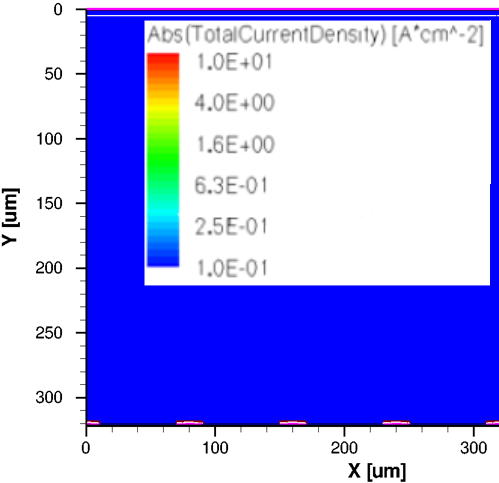
\includegraphics[width=0.31\textwidth]{figures/silicon/silicon_t0.0.png}
  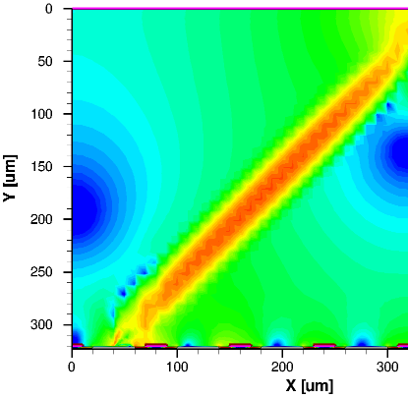
\includegraphics[width=0.31\textwidth]{figures/silicon/silicon_t1.1.png}
  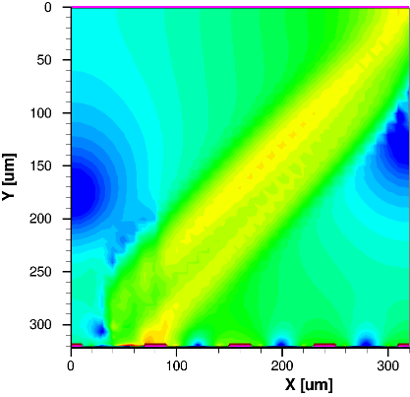
\includegraphics[width=0.31\textwidth]{figures/silicon/silicon_t1.5.png}\\
  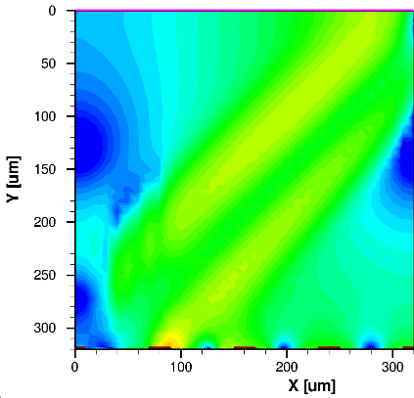
\includegraphics[width=0.31\textwidth]{figures/silicon/silicon_t2.0.png}
  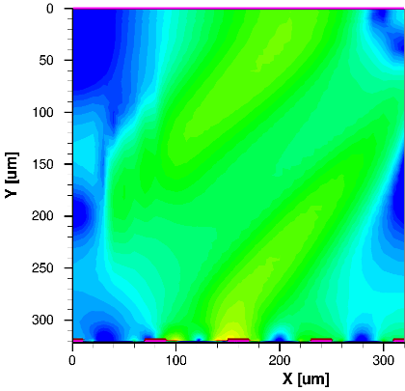
\includegraphics[width=0.31\textwidth]{figures/silicon/silicon_t3.0.png}
  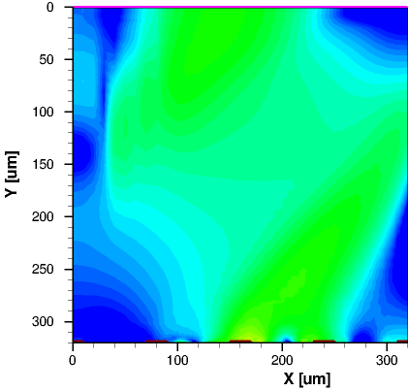
\includegraphics[width=0.31\textwidth]{figures/silicon/silicon_t4.0.png}\\
  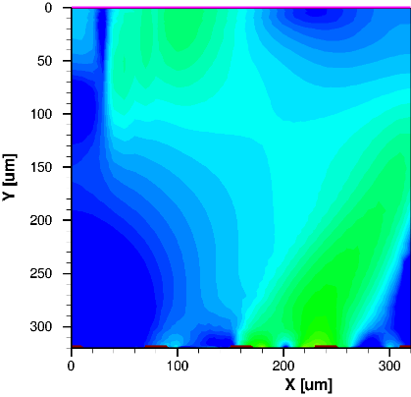
\includegraphics[width=0.31\textwidth]{figures/silicon/silicon_t5.0.png}
  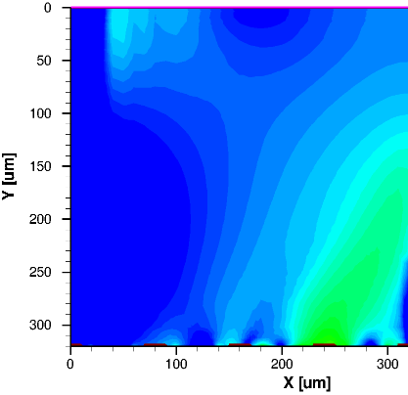
\includegraphics[width=0.31\textwidth]{figures/silicon/silicon_t6.0.png}
  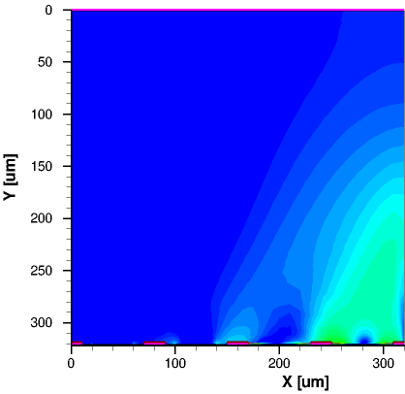
\includegraphics[width=0.31\textwidth]{figures/silicon/silicon_t7.0.png}\\
    \caption{\label{fig:sd} (simulation) MIP particle traveling across a silicon strip sensor at $45^\circ$ over time from 0.0, 1.1,1.5,2,3,4,5,6,7 nanoseconds. The induced surface current dissapates and would be collected by the channels of the silicon module ~\cite{Eichhorn:2112017}.}
\end{figure}





\subsubsection{Pixel Detector}
\label{sec:pixeldet}
The pixel detector contains the Barrel Pixels (BPIX) and the Forward Pixels (FPIX).  
Similar $2\times8$ silicon detector modules make up both the BPIX and FPIX systems.

In 2016, the phase 1 Forward Pixel System (FPIX) was constructed and tested. At Purdue University, an Aerotech robotic gantry control system was used to join a hybrid flex circuit to a bump-bonded silicon pixel module. After wirebonding, the gantry system encapsulated the wirebonds for protection from corrosion and magnetic field resonance. Purdue was one of the manufacturing sites alongside University Nebraska-Lincoln. 

Using LabVIEW, we developed a state machine to assemble and encapsulate these pixel modules. Pattern recognition and a linear algebra suite were developed to perform precise operations at a 50 micron resolution. An example of a post encapsulated token bit manage--which resides on top of the high density interconnect of a completely assembly module---is shown in figure \ref{fig:tbm}.

\begin{figure}[ht!b]
    \centering
  \includegraphics[width=0.65\textwidth]{fpixtbm.jpg}
    \caption{\label{fig:tbm} encapsulated token bit manager of a forward pixel module currently installed in CMS}
\end{figure}


In 2017, this system was installed in CMS, increasing the number of disks to three and the number of barrel layers to four.  The design of CMS is such that the inner sub-detector systems may be taken out of the solenoid and serviced.  
These forward disks, which are especially important for the reconstruction of boosted charged particles, are located in high regions of $\eta$ and are overlapped for improved hermeticity.  


\subsubsection{Silicon Tracker}
The silicon tracker comprises larger silicon modules by area than the pixel system and is located further from the beam pipe. A representative layout of the silicon tracker and the pixel system can be found in figure \ref{fig:tracker} ~\cite{Chatrchyan:2008zzk}. 

\begin{figure}[ht!b]
\label{fig:tracker}
  \centering
  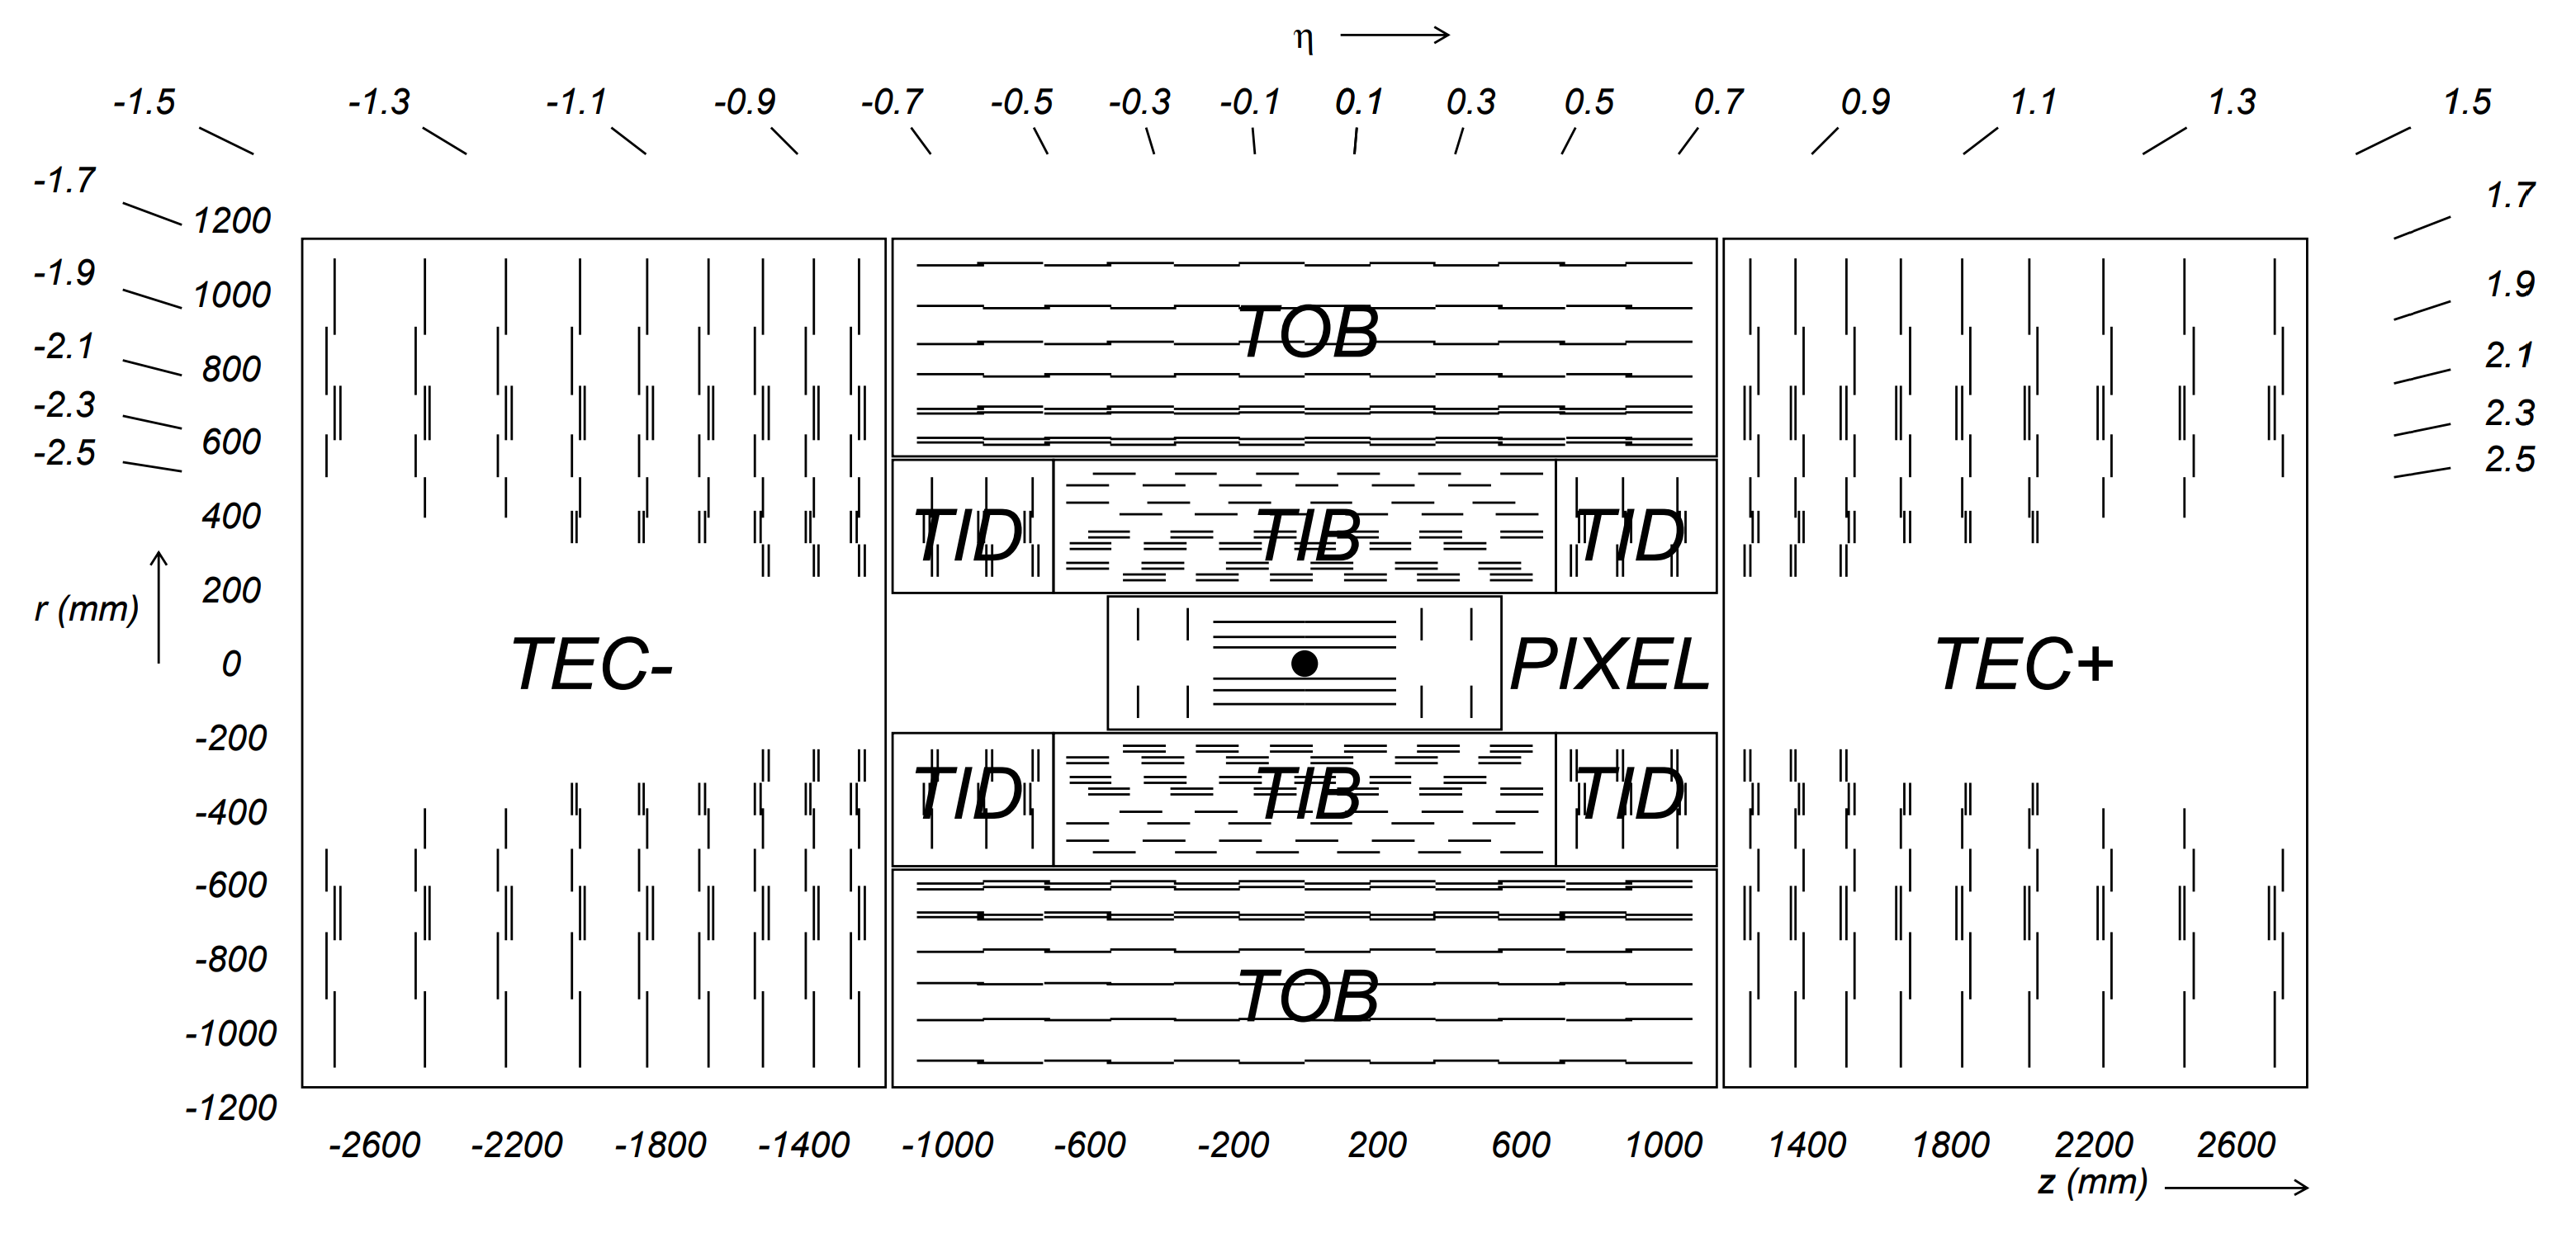
\includegraphics[width=0.85\textwidth]{figures/silicon/SiliconTracker.png}\\
    \caption{ The silicon tracker system, consisting of the inner pixel system (BPIX and FPIX), The Tracker End Caps (TEC), Tracker Inner Detector(TID), Tracker Inner Barrel (TIB), and the Tracker Outer Barrel (TOB) by position in r, z , and $\eta$ ~\cite{Chatrchyan:2008zzk}}
\end{figure}



\subsection{Electromagnetic Calorimeter (ECAL)}

The principal components of the ECAL are the 76200 lead tungstate ($\text{PbWO}_4$) crystals, which scintillate and absorb energy from incoming particles. These detector components are also separated in barrel and endcap regions. A photomultiplier is attached to each the crystal to detect its light signal. The relative energy resolution is 
\begin{equation*}
\label{eq:ecal}
\left(\frac{\sigma}{E}\right)^2 = \left( \frac{2.8\%}{\sqrt{E}}  \right)^2 + \left( \frac{0.12}{E}  \right)^2 + (0.3\%)^2 
\end{equation*}
 The first, second, and third terms in equation \ref{eq:ecal} reflect the stochastic, noise, and constant terms as determined in the calibration run with a 440 nm blue laser ~\cite{Chatrchyan:2008zzk,Eichhorn:2112017}. 

\subsection{Hadronic Calorimeter (HCAL)} 
The Hadronic Calorimeter is the primary sub-detector to identify ``jets", which are collimated collections of hadrons. 
Brass plates interwoven with plastic scintillator are used to induce particle showers. 
Light signals from the scintillators are read out using photodetectors. % check 
There are barrel (HB) and endcap (HE) inside the solenoid. The Hadronic Outer (H0) and super forward detector (HF) sit outside the solenoid. An overview of the HCAL system is shown in figure \ref{fig:hcal} ~\cite{Chatrchyan:2008zzk,Eichhorn:2112017}. 

\begin{figure}[ht!b]
  \centering
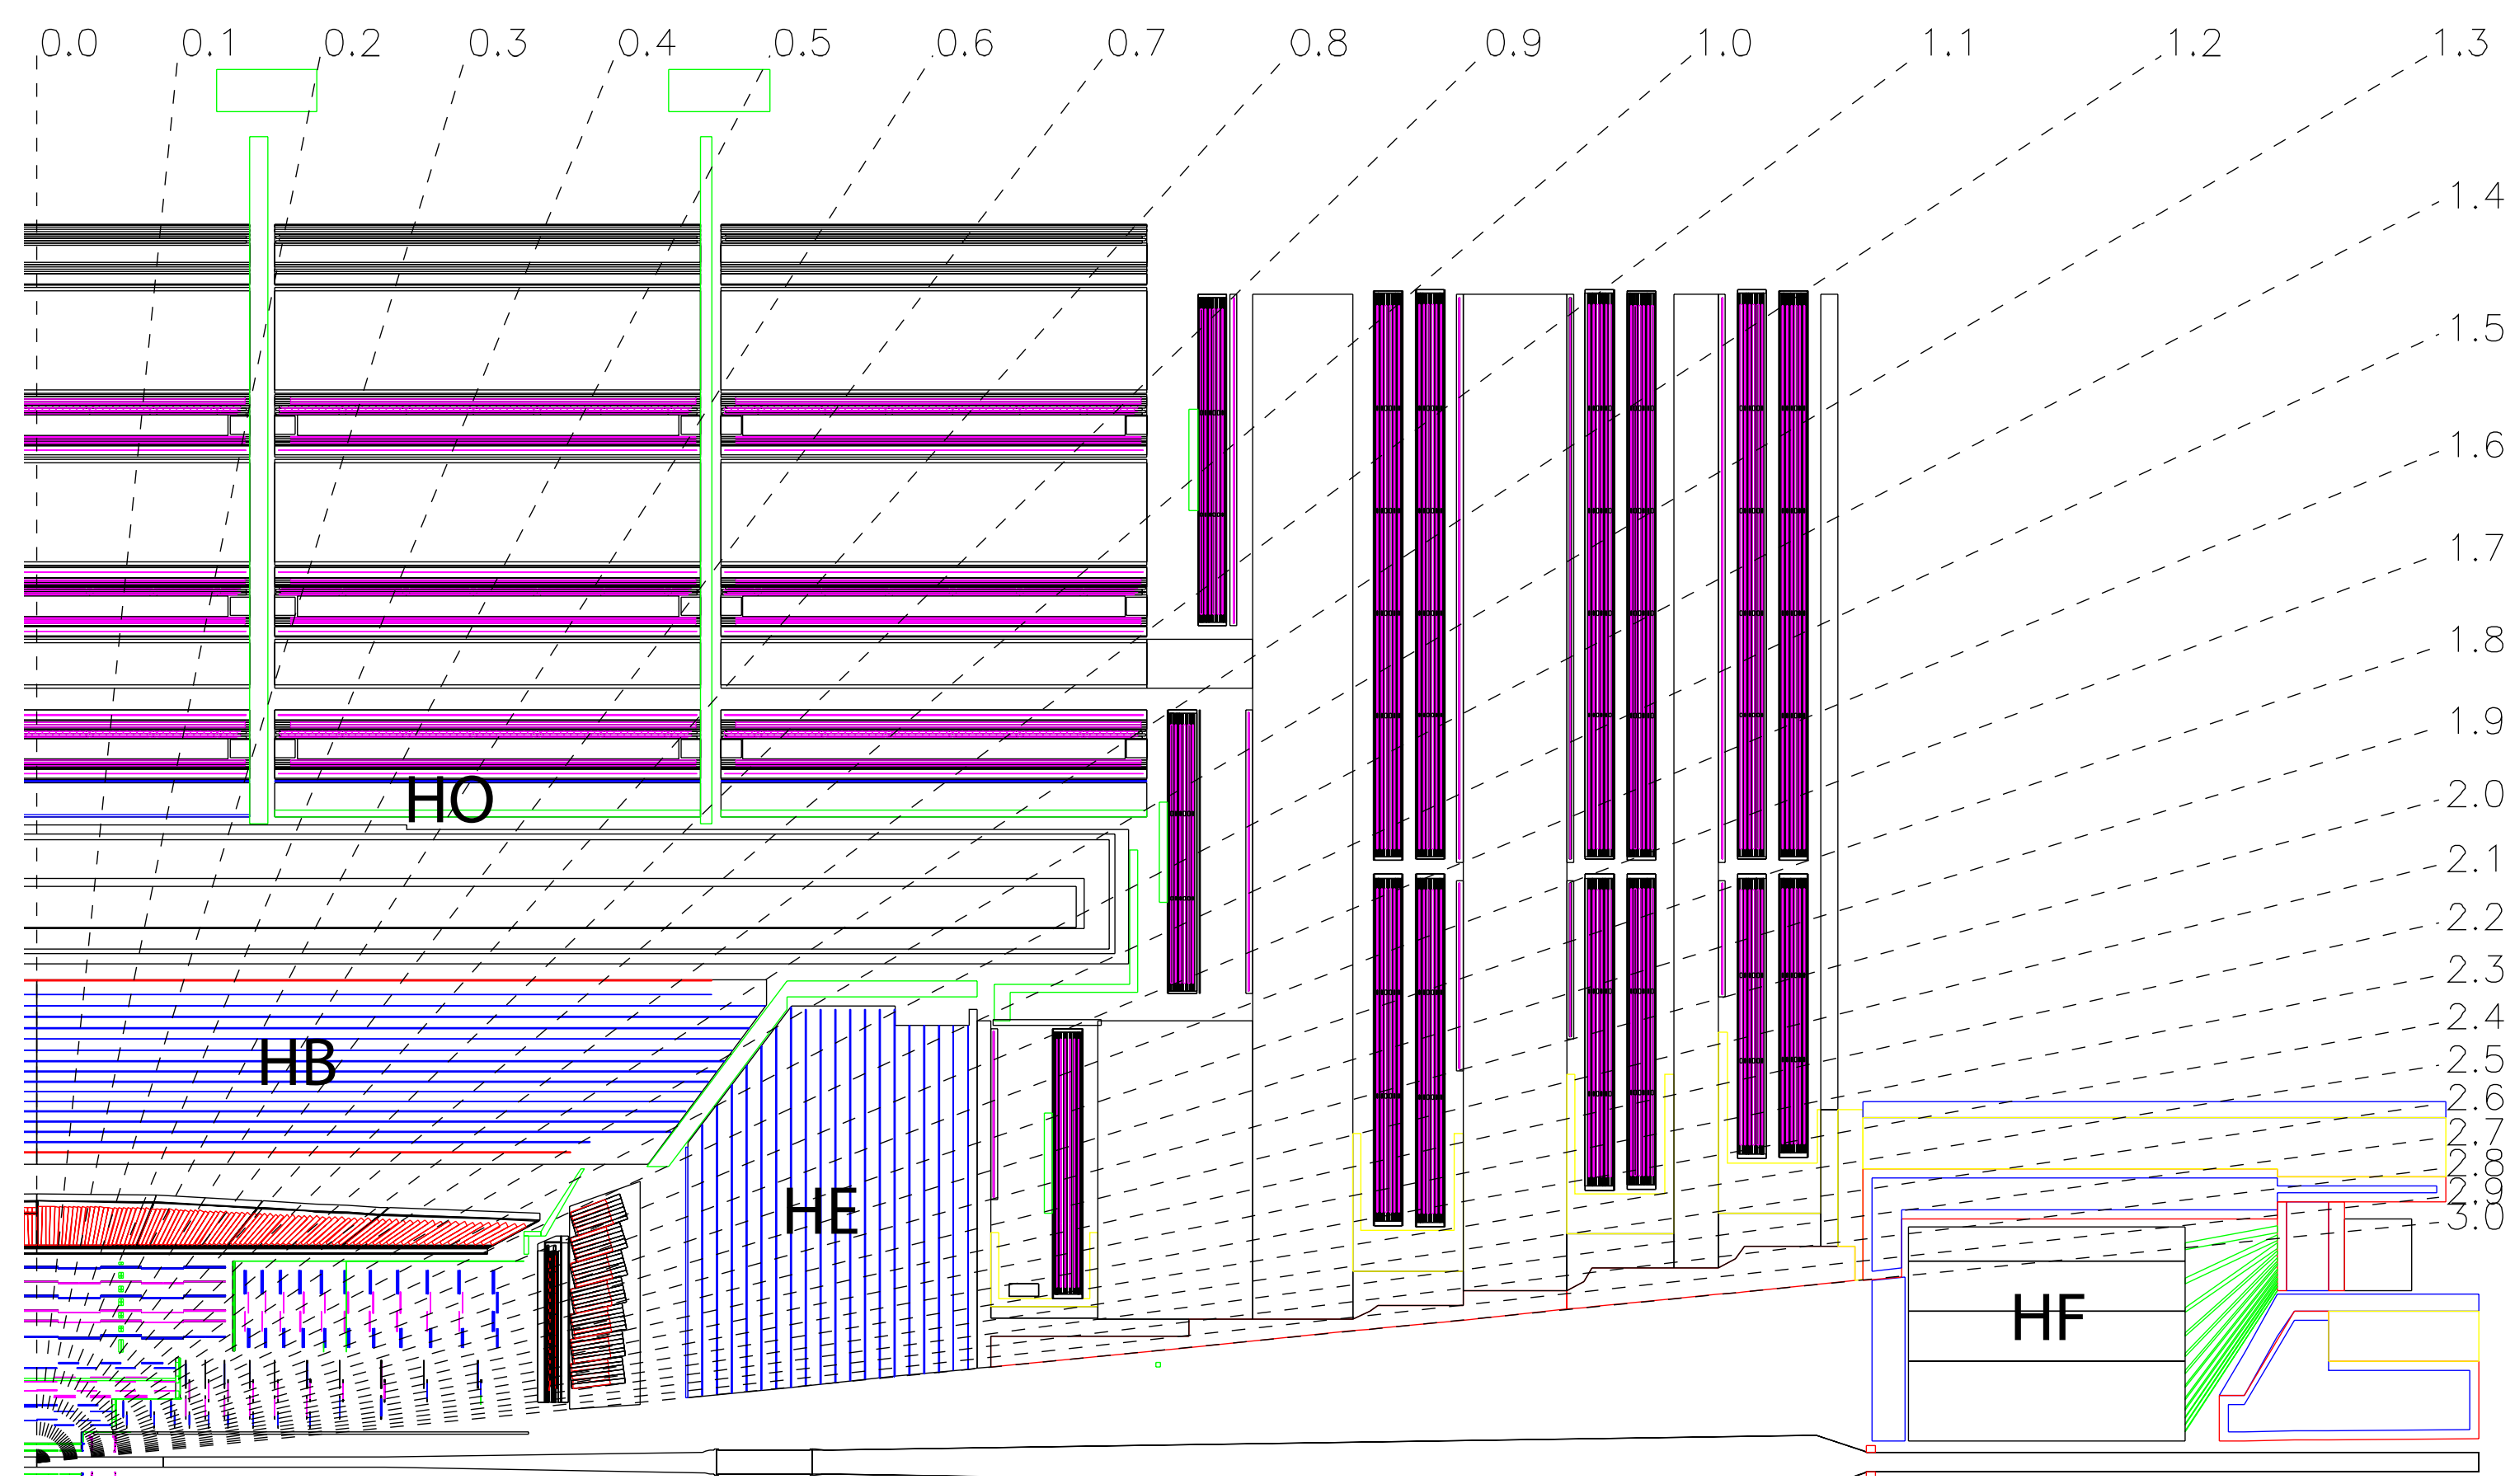
\includegraphics[width=0.85\textwidth]{figures/HCAL.png}    
    \caption{\label{fig:hcal} Overview of the HCAL system from the z---$\eta$ plane showing the hadron barrel (HB), encap(HE), outer (HO), and the forward (HF) subsystems ~\cite{Chatrchyan:2008zzk}}
\end{figure}




\subsection{Muon System} 
The muon system comprises drift tubes which cover a pseudorapidity region ($|\eta|<1.2$) split into four stations interleaved in the flux return plates.
In the higher $|\eta|$ endcap regions, cathode strip chambers (CSCs), which provide fast response time, fine segmentation, and radiation resistance, are used ~\cite{Chatrchyan:1129810}. For a visual representation of a cross section of the muon system please refer to figure ~\ref{fig:muonsystem}. 
Notably, the track of the muon is bent inside the solenoid by the Lorentz force, and then reverses after it exits. 

\begin{figure}[ht!b]
  \centering
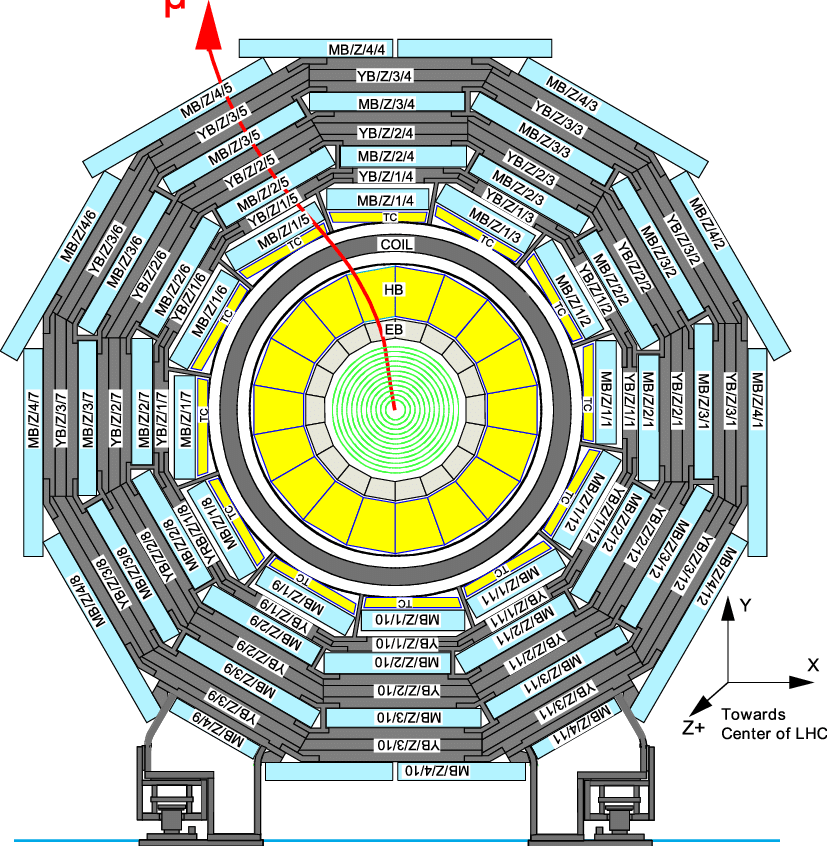
\includegraphics[width=0.75\textwidth]{figures/Layout-of-the-CMS-barrel-muon-DT-chambers-in-one-of-the-5-wheels-59.png}    
    \caption{\label{fig:muonsystem} Muon system involving multiple subdetector systems: tracker, solenoid, and the muon gas chambers around the iron yoke (grey) - Maximilien Brice, CERN }
\end{figure}


\section{Level 1 Trigger System and High Level Trigger}
Particle collisions happen at a rate of 40 MHz with each bunch crossing, resulting in about 20 minimum bias events. The bandwidth that would be needed to record all these collisions is prohibitively high ~\cite{Bruning:782076,Foudas:2232067}. The Level 1 trigger (L1) and High Level Trigger (HLT) work to reduce these rates by selecting events of interest. 

The L1 trigger system, which comprises many subsystems,can process data at the beam collision rate. Algorithms are in place that take input from the calorimeters, the muon systems, and other detectors in the form of ``trigger primitives'' and use pattern recognition, along with fast summing techniques, to trigger on the event. Many of these algorithms are run on Field Programmable Gate Arrays (FPGAs). 
After 144 beam crossings, the Global Trigger (GT) initiates readout for events of interest at the front end electronics. 
 The L1 system also outputs physics objects to seed the reconstruction algorithms used by the HLT ~\cite{Foudas:2232067}. 
The HLT maximum input rate is 100~kHz and the output is on the order of kHz. It is constrained by the processing power available, the data recording and transfer rate of Tier 0, and the prompt reconstruction algorithms. Late in Run II  ``Scouting'' and ``Parking'' data were used to make more efficient use of the available bandwidth. Scouting reduces the event size by saving only objects reconstructed by the HLT. Parking reduces the immediate load on the T0 system by postponing prompt reconstruction to a time when CMS is not running ~\cite{Thomas:2703017}.


\section{Particle Flow Algorithms}
The event data model requires association of higher level physics objects---like leptons---with energy deposits and tracks in the detector. 
The particle flow algorithm at CMS has the goal of associating these primary detector signatures with these particles so that direct comparison to Monte Carlo simulation can be done. 
The list of particle objects includes jets, missing transverse energy, taus, charged-leptons, photons, and bottom quark jets among others.
To outline the algorithm: charged particle tracks reconstructed in the tracker, energy clusters from the ECAL, HCAL, and preshower detector (ES), and forward calorimeter (HF) are topologically linked into blocks. The linking is done through many associations of energy deposits and tracks in $\phi,\eta$ space. These blocks are then interpreted as particles. Further details can be found in reference ~\cite{CMS-PAS-PFT-10-001}.

\section{Computational Infrastructure}
Over 200 peta-bytes of information have been gathered in Run II. A schematic overview of the computing infrastructure can be found in figure \ref{fig:t0} ~\cite{Hufnagel:1319049}.

\begin{figure}[ht!b]
  \centering
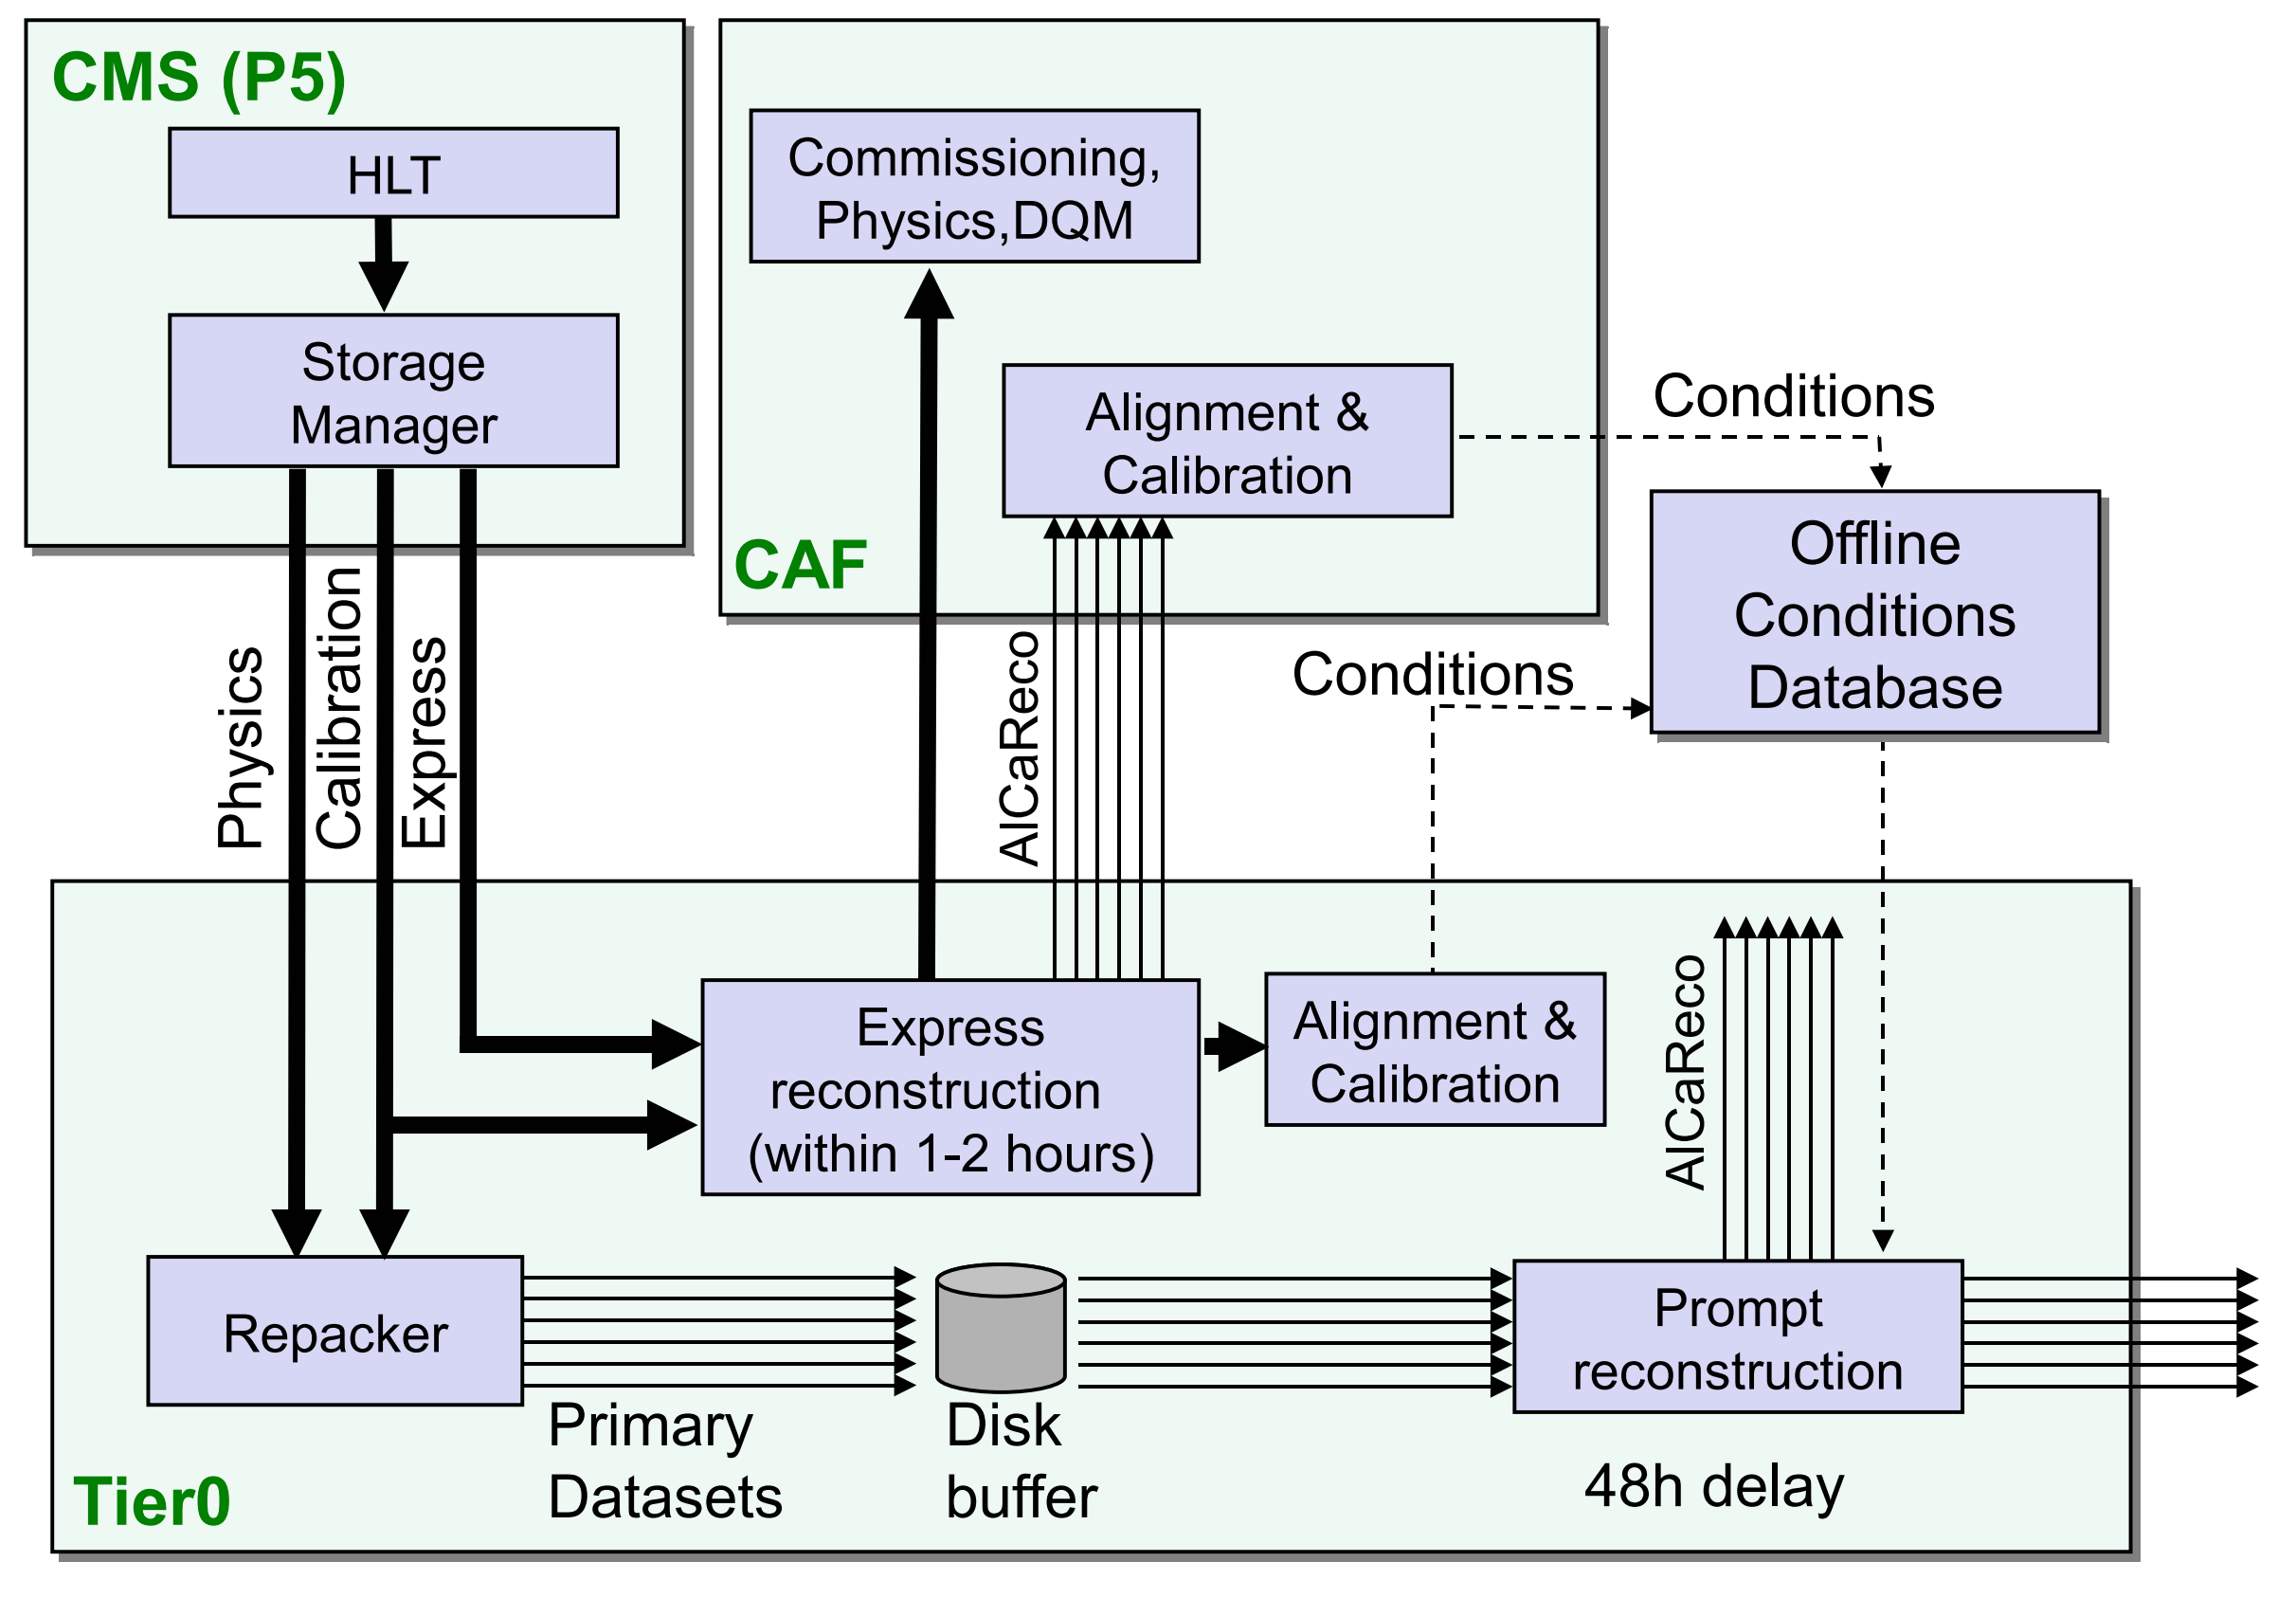
\includegraphics[width=0.75\textwidth]{figures/Tier0.png}    
    \caption{\label{fig:t0} Schematic overiew of Tier0 computing, data can be available from different sections allowing for data quality monitoring and also storage to several databases ~\cite{Hufnagel:1319049} }
\end{figure}

The Tier 0 (T0) facility which comprises 32,000 24-core processors is where higher level reconstruction of physics objects is done.  
The data are stored and processed at many different sites, organized by tiers. There is one Tier-0, seven Tier-1, about one-hundred fifty Tier-2, and numerous Tier-3 centers. The sum of these tiers is the ``grid'' or the Worldwide LHC Computing Grid (WLCG), which in total combines 900 000 CPUs from over 170 sites in 42 countries. Tools like \texttt{XrootD} and \texttt{Rucio} allow physicists from around the world to access centrally supported data. An abundance of up to date information can be found \texttt{https://home.cern/science/computing/grid}. 



